\section{Numerical Methods}

\subsection{Question 3}

The numerical integrator with and functions for both Euler's and Heun's methods of integration is in  the file \texttt{numerical\_integration.jl}. The SIS model and the solutions are in a notebook \texttt{sis\_model.ipynb}. For all practical purposes discrete time models are identical to numerical solutions to continuous equations. The only difference is the inclusion of the term $\Delta T$ in the latter which does not necessarily need to appear in the former.


\subsection{Question 4}

The SIS model has the following form
\begin{equation}
\label{eqn:heuns_def}
\begin{cases}
\dot{S} = -\beta S I + \gamma I \\
\dot{I} = \beta S I - \gamma I
\end{cases}
\end{equation}

Where S is the number of susceptible individuals in the population, I is the number of infected individuals, $\beta$ is the infection rate and $\gamma$ is the recovery rate.

The equations are numerically solved with two algorithms. First, is Euler's method:

\begin{equation}
x_e(t+x) = x(t)+f(x(t))h
\end{equation}

Secondly, the results are calculated using Heun's method. Heun's method is more accurate and has a global error $\mathcal{O}(h^2)$

\begin{equation}
\label{eqn:heuns_def}
x_h(t+h) = x(t)+\frac{h}{2} [\ f(x_e(t+x))+f(x(t)]\
\end{equation}

The solutions to the SIS model using Heun's method are displayed in Fig. \ref{fig:SIS_results}. Each run is run until a max time of $T=10$ regardless of the number of steps the integrator takes. This allows us to compare the behavior of the algorithm at the same scale, regardless of the 


For the smallest step size of 0.01, the two methods diverge only slightly across all three values of $\beta$. Increasing values of $\beta$ increase the rate at which S drops. The difference in the algorithms can be most clearly seen in $ step\_size: 0.5|\beta = 0.03$. Here, Heun's method remains smooth while visible artifacts from the integration are seen with Euler's method. The strangest result is $step\_size: 0.5|\beta = 0.06$. Here, Heun's method oscillates between two values while Euler's method appears to be chaotic. The behaviors here are reminiscent of the behavior of the logistic map, with Heun's method analogous to the logistic map oscillating between two values and Euler's method being analogous to chaotic behavior of the logistic map. Since both numerical integration of the SIS model and the logistic map are discrete time models, it is plausible there is a formal connection. 




\begin{figure}[h]
  \centering
  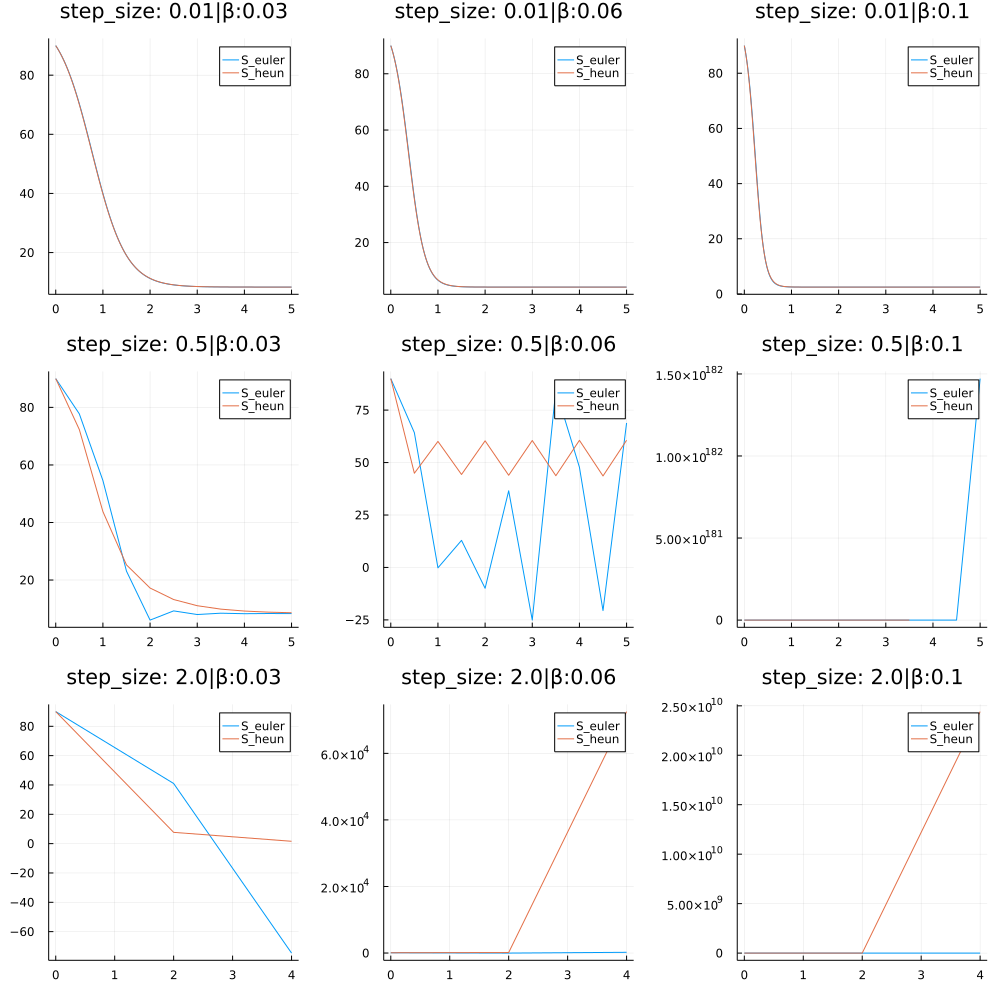
\includegraphics[width = \textwidth]{fig/euler_heun_comp.png}
  \caption {The results of numerical integration of the SIS model with Euler's method and Heun's method. Results for S are plotted for step sizes 0.01,0.5 and 2.0 and for values of $\beta$ 0.03,0.06,0.1}
  \label{fig:SIS_results}
\end{figure}




\subsection{Question 5}

\begin{quote}
Show that the global error of Heun's method is of order $h^2$
\end{quote}

We will begin with the definition of Heun's Method 

\begin{equation}
\label{eqn:heuns_def}
x_h(t+h) = x(t)+\frac{h}{2} [\ f(x_e(t+x))+f(x(t)]\
\end{equation}

Where $x_e(t+h)$ is Euler's method at point $t+h$

\begin{equation}
x_e(t+x) = x(t)+f(x(t))h
\end{equation}

Now for small values of h($h << 1$) we can make the approximation that 

\begin{equation}
\label{eqn:heun_approx}
f(x_e(t+h)) \approx (x(t+h))
\end{equation}

This is equivalent to assuming that for small step sizes, Euler's method predicts the correct next point in the function. 
We also assume the derivative is linear and can be distributed.
\begin{equation}
\label{eqn:approx_2}
f((x(t+h))) = \frac{d}{dt}f(x(t+h)) = f(x(t))+hf'(x(t))
\end{equation}

We substitute eq. \ref{eqn:approx_2} into eq. \ref{eqn:heuns_def} to find the following: 

\begin{equation}
\label{eqn:heun_sub}
x_h(t+h) = x(t)+\frac{h}{2} [\ f(x(t))+hf'(x(t))+f(x(t))]\
\end{equation}

Collecting terms and simplifying

\begin{equation}
\label{eqn:heun_sub_simp}
x_h(t+h) = x(t)+hf(x(t))+\frac{h^2}{2}f'(x(t))
\end{equation}

Which is exactly equivalent to the first three terms of the taylor expansion of $x(t)$

\begin{equation}
\label{eqn:taylor_2}
x(t+x) = x(t)+hf(x(t))+\frac{h^2}{2} f'(x(t))+\mathcal{O}(h^3)
\end{equation}

So Heun's method is equivalent to the correct time evolution up to terms of order $h^3$. This means that heun's mathod has a local error $\mathcal{O}(h^3).$


$Global Error = LocalError\times TimeSteps$ But $TimeSteps = \frac{T}{h}$ Where $T$ is the total time and $h$ is the step size. 
As a result 
\begin{equation}
\label{eqn:taylor_2}
Global Error \propto \frac{\mathcal{O}(h^3)}{h} = \mathcal{O}(h^2)
\end{equation}

QED

